\chapter{Methodology}
\label{methodology}

\section{Requirements}
\label{methodology:s:requirements}

\subsection{Current Architecture}
\label{methodology:ss:current-architecture}

The current software architecture is still in use as of the date of publication of this body of work. This older architecture consists of an amalgamation of Docker containers, each running a different service. Each Client has its own, \gls{vps}, wherein these Docker containers are deployed. 

These \gls{vps} are general-purpose \gls{aws} \gls{ec2} \textit{Instances}. As can be seen on the diagram presented on \Cref{fig:old-arch-overview.drawio.pdf}, these instances are deployed to the same \gls{vpc}, sharing a private network between them. The Reverse Proxy serves as, as the name implies, as a reverse proxy to enable the use of a single \gls{eip}, a single \gls{nic} by all Clients's servers, since the availability of public IPs is limited to five \gls{eip}.
\begin{figure}[!htbp]
    \centering
    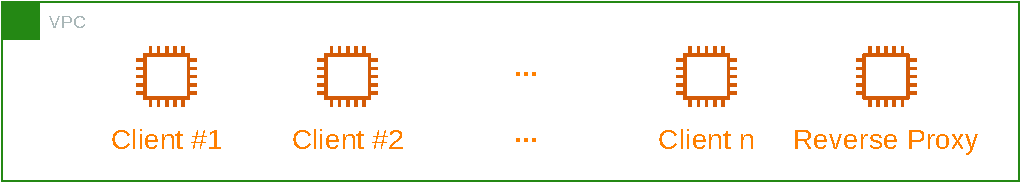
\includegraphics[width=0.90\textwidth]{img/diagrams/pdf/old-arch-overview.drawio.pdf}
    \caption[AWS VPC Overview]{The AWS VPC used, hosting the old architecture's EC2 \gls{vps}.}
    \label{fig:old-arch-overview}
\end{figure}
    

Each VPS runs a Docker container for each one of the following services:

\begin{itemize}

\item \textbf{InfluxDB} (Timeseries Database)
\item \textbf{MongoDB} (General use, no-SQL, Document Database)
\item \textbf{Grafana} (Web platform for data visualization, the front end of the \gls{dss})
\item \textbf{Telegraf} (Data collecting service)
\item \textbf{Nginx} (Reverse proxy with HTTPS capabilities)
\item \textbf{Let's Encrypt} (Automatic SSL Certificate emitter, companion for the Nginx container)
\item \textbf{Web Dev} (Web platform / API for managing Workers' settings)
\item \textbf{Redis} (Message Queue System for queuing Worker's jobs)
\item \textbf{OpenSSH} (\textit{atmoz/sftp}) (SFTP Server for receiving client data)
\item \textbf{Workers} (Container running the Forecast, Simulation and Optimization Python Algorithms as well as the KPI Algorithms.)
\item \textbf{Workers} (\textit{Beat}) (Container that periodically \textit{triggers} jobs in the Workers container)

\end{itemize}

\begin{figure}[!htbp]
    \centering
    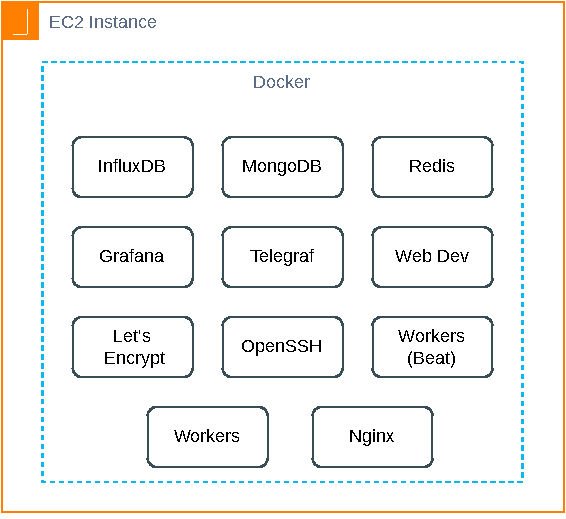
\includegraphics[width=0.75\textwidth]{img/diagrams/pdf/old-arch.drawio.pdf}
    \caption[AWS EC2 VPS Overview]{An AWS EC2 VPS, hosting the old architecture's docker containers}
    \label{fig:old-arch.drawio.pdf}
\end{figure}
    


\subsubsection{Databases}
\label{methodology:sss:databases}

There are two types of databases being used by this architecture: A Timeseries Database, in this case \textbf{InfluxDB}, and an additional general-purpose Document Database: \textbf{MongoDB}. Each type of database has a different role, the first one stores the Client's timeseries data such as sensor information, pump orders, predicted tank levels, etc.
The second one, the Document Database, is responsible for storing configuration settings for each worker service (optimization, simulation and forecasting), for storing electrical tariffs data and to store sensor device's configurations.

\subsubsection{Grafana}
\label{methodology:sss:grafana}

This web platform allows the visualization of the Timeseries data from the \textbf{InfluxDB} database. This is a freely-available platform that runs on a docker container with little to no modifications necessary. The dashboards are built using the built-in tools and allow for complex and very informative data visualization. This is used in both the new and old architecture, since the new visualization platform is still not operational (not within the scope of this body of work).

\subsubsection{Telegraf}
\label{methodology:sss:telegraf}

The \textbf{Telegraf} container is used to gather the files containing the raw sensor data sent from the Client to the \textbf{SFTP} server. Since this container shares the file upload location folder with the \textbf{SFTP}, through a convoluted process of storing the filename of the last file uploaded, periodically checking for the next file and file handling \textit{spaghetti} code that spans multiple files and has an enormous codebase that weighs the docker image's file size considerably. 